\chapter{Axiomatizing Valid General Concept Inclusions of Finite
  Interpretations}
\label{cha:axiom-valid-el}

Our considerations about extracting general concept inclusions from erroneous data will be
based on previous results obtained by \textcite{Diss-Felix} on extracting all \emph{valid}
general concept from finite interpretations.  We shall therefore review in this section
all necessary notions from this work that are needed for our own.

The problem of extracting all valid general concept inclusions from a finite
interpretation can be made more precise as follows.  Let $\mathcal{I} =
(\Delta^{\mathcal{I}}, \cdot^{\mathcal{I}})$ be a finite interpretation over $N_C$ and
$N_R$, \ie $\Delta^{\mathcal{I}}$ is a finite set.  The task is then to find the set of
all general concept inclusions $C \sqsubseteq D$ with $C, D \in \ELbot(N_C, N_R)$ which
are valid in $\mathcal{I}$.

Of course, this set is infinite of valid general concept inclusions in general.  This is
because if $C \sqsubseteq D$ holds in $\mathcal{I}$, and $r \in N_R$, then $\exists r. C
\sqsubseteq \exists r. D$ holds in $\mathcal{I}$ as well.  Such an infinite set is hardly
usable to represent knowledge suitable for machine consumption.  Therefore, the
considerations in~\cite{Diss-Felix} concentrate on finding \emph{finite bases} of
$\mathcal{I}$, \ie set of valid general concept inclusions of $\mathcal{I}$ which are also
\emph{complete}.  We shall introduce these notions briefly in \Cref{sec:bases-gener-conc}.

One of the main results of~\cite{Diss-Felix} is then that finite bases for finite
interpretations $\mathcal{I}$ always exist, and we shall discuss them in
\Cref{sec:base-all-valid}.  These results have been obtained by exploiting a close
connection between description logics and formal concept analysis.  It is therefore
crucial that we introduce this connection first, and we shall do so
in~\Cref{sec:motivation}.  In particular, we shall talk about \emph{induced contexts} and
\emph{model-based most-specific concept descriptions}.

In what follows, we shall fix the two disjoint sets $N_C$ and $N_R$ and shall not mention
them explicitly anymore.  This means, for example, that whenever we are talking about
interpretations or concept descriptions, we are actually talking about interpretations
over $N_C$ and $N_R$, and about concept descriptions over $N_C$ and $N_R$.

\section{Bases of General Concept Inclusions}
\label{sec:bases-gener-conc}

General concept inclusions have a \emph{model-based semantics}, their semantics is defined
in terms of being valid in some interpretation.  We can therefore introduce a notion of
\emph{entailment} and \emph{completeness}, much like as we did for implications.

\begin{Definition}
  \label{def:entailment-of-gcis}
  Let $\mathcal{L} \cup \set{ C \sqsubseteq D }$ be a set of general concept inclusions
  over $N_C$ and $N_R$.  We shall say that $\mathcal{L}$ \emph{entails} $C \sqsubseteq D$,
  written $\mathcal{L} \models (C \sqsubseteq D)$ if and only if for all interpretations
  over $N_C$ and $N_R$ it is true that if $\mathcal{I} \models \mathcal{L}$, then
  $\mathcal{I} \models \set{ C \sqsubseteq D }$ as well.

  Let $\mathcal{K}$ be another set of general concept inclusions over $N_C$ and $N_R$.
  Then $\mathcal{K}$ is said to be \emph{sound} for $\mathcal{L}$ if and only if all
  general concept inclusions in $\mathcal{K}$ are entailed by $\mathcal{L}$.
  $\mathcal{K}$ is said to be \emph{complete} for $\mathcal{L}$ if and only if all general
  concept inclusions in $\mathcal{L}$ are \emph{entailed} by $\mathcal{K}$.  $\mathcal{K}$
  is said to be a base for $\mathcal{L}$ if and only if $\mathcal{K}$ is sound and
  complete for $\mathcal{L}$.
\end{Definition}

Notice the similarity of this definition to \Cref{def:sound-complete-base}.

Let $\mathcal{I}$ be a finite interpretation over $N_C$ and $N_R$, and let us denote with
$\Th_{\ELbot(N_C, N_R)}(\mathcal{I})$ the set of all \ELbot general concept inclusions
over $N_C$ and $N_R$ which are valid in $\mathcal{I}$, and likewise denote with
$\Th_{\ELgfpbot(N_C, N_R)}(\mathcal{I})$ the set of all \ELgfpbot general concept
inclusions over $N_C$ and $N_R$ which are valid in $\mathcal{I}$.  If the logic used is
clear from the context, then we shall drop the subscript.

Let $\mathcal{K}$ be a set of general concept inclusions over $N_C$ and $N_R$.  If
$\mathcal{K}$ is a set of \ELbot general concept inclusions and is a base for
$\Th_{\ELbot(N_C, N_R)}(\mathcal{I})$ we shall simply say that $\mathcal{K}$ is an
\emph{\ELbot base} of $\mathcal{I}$.  If we replace \ELbot by \ELgfpbot, then we call
$\mathcal{K}$ an \emph{\ELgfpbot base} instead.  If the logic is clear from the context or
not relevant for the current consideration, we shall leave it out.

Notice that in the case that $\mathcal{K}$ is an \ELbot base of $\mathcal{I}$, all general
concept inclusions in $\mathcal{K}$ have to hold in $\mathcal{I}$: the set
$\Th(\mathcal{I})$ is \emph{closed under entailment} in the sense that every \ELbot
general concept inclusion over $N_C$ and $N_R$ which is entailed by $\Th(\mathcal{I})$ is
already contained in this set.  Therefore, if $\mathcal{K}$ is sound for
$\Th(\mathcal{I})$, it must be contained in this set and thus $\mathcal{K}$ is a set of
general concept inclusions which are valid in $\mathcal{I}$.  Moreover, since
$\mathcal{K}$ is complete for $\Th(\mathcal{I})$, every general concept inclusion over
$N_C$ and $N_R$ that holds in $\mathcal{I}$ is entailed by $\mathcal{K}$.

\section{Linking Formal Concept Analysis and Description Logics}
\label{sec:motivation}

Description logics and formal concept analysis are connected by a number of similar
notions.  As an example, let us consider a formal context $\con K = (G, M, I)$ and a set
$A \subseteq M$.  Then the set $A'$ is the set of all objects of $\con K$ which have all
the attributes in $A$.  We can view this fact from another perspective: if $A = \set{ m_1,
  \dots, m_n }$, then we can think of the attributes $m_1, \dots, m_n$ as
\emph{propositions}, and the fact that $(g, m) \in I$ as saying that $g$ \emph{satisfies}
the proposition $m$.  Then $g \in A'$ means that $g$ \emph{satisfies} the conjunction of
all propositions in $A$.

Let us reformulate this using description logics, and let us define $N_C := M$ and $N_R =
\emptyset$.  Then we can think of $\con K$ as an interpretation $\mathcal{I}_{\con K} =
(G, \cdot^{\mathcal{I}_{\con K}})$ where
\begin{equation}
  \label{eq:17}
  m^{\mathcal{I}_{\con K}} := \set{ g \in G \mid (g, m) \in I } = \set{ m }'.
\end{equation}
Then indeed we have that $A' = (m_1 \sqcap \dots \sqcap m_n)^{\mathcal{I}_{\con K}}$ for
all finite $A = \set{ m_1, \dots, m_n } \subseteq M$.  Indeed, if we would consider a
description logic that only allows for conjunction $\sqcap$, then we can view finite
formal contexts, derivation of sets of attributes and even implications as special cases
of finite interpretations, extensions of concept descriptions and general concept
inclusions.  Thus the derivation operator $(\cdot)' \colon \subsets{M} \to \subsets{G}$
corresponds naturally to computing the extension of concept descriptions in
interpretations.  However, the other derivation operator $(\cdot)' \colon \subsets{G} \to
\subsets{M}$ does not have such a correspondence in description logics.  This gap shall be
filled by considering \emph{model-based most-specific concept descriptions}, which we
introduce in \Cref{sec:defin-and-basic}.

The connection between description logics and formal concept analysis expressed in
\eqref{eq:17} only works in one direction: it allows to represent basic notions of formal
concept analysis in terms of description logics, but not vice versa.  Even if we restrict
our attention to the rather light-weight description logic \ELbot, it is not clear how to
represent an interpretation by means of notions from formal concept analysis.

To approach this issue, we shall introduce \emph{induced contexts} in
\Cref{sec:induced-contexts}.  Such contexts allow to express tight connections between the
notions of formal concept analysis and description logics, and, since induced contexts are
just formal contexts, still allows the application of standard methods from formal concept
analysis, such as the extraction of bases.  This fact will be exploited when we discuss
the computation of finite bases of in \Cref{sec:base-all-valid}.

\subsection{Model-Based Most-Specific Concept Descriptions}
\label{sec:defin-and-basic}

Let $\con K = (G, M, I)$ and Let us try to motivate how to find a natural correspondence
of the derivation operator $(\cdot)' \colon \subsets{G} \to \subsets{M}$ within
description logics.  Let $B \subseteq G$ be a set of objects of $\con K$.  Then the set $A
:= B'$ can be thought of as the \emph{most-specific} set of attributes that
\emph{describe} $B$, \ie
\begin{enumerate}[i. ]
\item $B \subseteq A'$, \ie $A$ \emph{describes} $B$, and
\item for all sets $C \subseteq M$ that satisfy $B \subseteq C'$ (that describe $B$) it is
  true that $C \subseteq A$, ($A$ contains \emph{more} attributes than $C$, \ie is
  \emph{more specific}).
\end{enumerate}
The last point is true because if $B \subseteq C'$, then by
\Cref{lem:derivation-is-galois-connection} it is true that $C \subseteq B' = A$.  Notice
that the description of $A$ as a most-specific description of $B$ is also a
characterization, \ie if $A$ is the most-specific description of $B$ in the above sense,
then $A = B'$.

To mimic this \emph{most-specific description} in description logics, Distel introduces
the notion of \emph{most-specific concept descriptions}.

\begin{Definition}[Most-Specific Concept Description]
  \label{def:most-specific-concept-description}
  Let $\mathcal{I} = (\Delta^{\mathcal{I}}, \cdot^{\mathcal{I}})$ be an interpretation, and
  let $X \subseteq \Delta^{\mathcal{I}}$.  A \emph{most-specific concept description} of
  $X$ in $\mathcal{I}$ is a concept description $C$ such that
  \begin{enumerate}[i. ]
  \item $X \subseteq C^{\mathcal{I}}$, and
  \item for each concept description $D$ satisfying $X \subseteq D^{\mathcal{I}}$ it is
    true that $C \sqsubseteq D$, \ie $C$ is subsumed by $D$.
  \end{enumerate}
\end{Definition}

If a model-based most-specific concept description $C$ for $X$ in $\mathcal{I}$ exists, it
is unique up to equivalence: if $D$ is another such model-based most-specific concept
description, than $C \sqsubseteq D$ and $D \sqsubseteq C$, by the last condition of the
definition.  Therefore, $C \equiv D$.  Because of this, we can talk about \emph{the}
model-based most-specific of $X$ in $\mathcal{I}$, and shall denoted it with
$X^{\mathcal{I}}$, to stress the similarity to the derivation operator from formal concept
analysis.  We shall also write $X^{\mathcal{I}\mathcal{I}}$ instead of
$(X^{\mathcal{I}})^{\mathcal{I}}$ and $C^{\mathcal{I}\mathcal{I}}$ instead of
$(C^{\mathcal{I}})^{\mathcal{I}}$ for syntactic convenience.

The existence of model-based most-specific concept descriptions, however, is not clear per
se, and the choice of the description logic in which we seek for model-based most-specific
concept descriptions is crucial here: if we only consider \ELbot concept descriptions,
then model-based most-specific concept descriptions do not necessarily exist, as is shown
in \Cref{expl:mmscs-may-not-exist-in-ELbot}.  However, if we allow all concept
descriptions in \Cref{def:most-specific-concept-description} to be \ELgfp or \ELgfpbot
concept descriptions, then the existence of model-based most-specific concept descriptions
can be guaranteed.

\begin{Theorem}[Theorem 4.7 of~\cite{Diss-Felix}]
  \label{thm:existence-of-mmscs-in-ELgfpbot}
  Model-based most-specific concept descriptions exist in \ELgfp and \ELgfpbot for all
  interpretations $\mathcal{I} = (\Delta^{\mathcal{I}}, \cdot^{\mathcal{I}})$ and sets $X
  \subseteq \Delta^{\mathcal{I}}$, and they can be computed effectively.
\end{Theorem}

The computation of model-based most-specific concept descriptions can be achieved using
\emph{\EL description graphs}, least common subsumers and
\emph{simulations}~\cite{DBLP:conf/ijcai/Baader03a,Diss-Felix}.  See~\cite[Section
4.1.2]{Diss-Felix} for details on this.

We have motivated model-based most-specific concept descriptions by most-specific
descriptions in formal contexts, and for this we have made use of the fact the derivation
operators form a Galois connection.  It is therefore only natural to expect that
model-based most-specific concept descriptions are also part of a Galois connection.
However, we have to notice that we cannot expect to obtain a Galois connection in the
sense of \Cref{sec:galois-connections}, simply because the relation $\sqsubseteq$ is not
antisymmetric, and thus not an order relation: it may be the case that $C \sqsubseteq D$
and $C \sqsubseteq D$, but $C \neq D$.  We can remedy this fact by considering concept
descriptions only \emph{up to equivalence}: instead of considering only a single concept
description $C$, we always consider the set $[C]$ of all concept descriptions which are
equivalent to $C$.  Then $[C] \sqsubseteq [D]$ is well-defined for all concept
descriptions $C$ and $D$, and $\sqsubseteq$ indeed yields an order relation this way.
This is only a technical detail, however, and we shall not make it explicit in our
following considerations.

\begin{Lemma}[Lemma 4.1 of~\cite{Diss-Felix}]
  \label{lem:mmsc-and-extension-are-galois-connection}
  Let $\mathcal{I} = (\Delta^{\mathcal{I}}, \cdot^{\mathcal{I}})$ be an interpretation
  over $N_C$ and $N_R$, $X \subseteq \Delta^{\mathcal{I}}$ and $C$ an \ELgfpbot concept
  description over $N_C$ and $N_R$.  Then
  \begin{equation}
    \label{eq:19}
    X \subseteq C^{\mathcal{I}} \iff X^{\mathcal{I}} \sqsubseteq C.
  \end{equation}
  In particular, for $X, Y \subseteq \Delta^{\mathcal{I}}$ and for \ELgfpbot concept
  descriptions $C, D$ over $N_C$ and $N_R$, it is true that
  \begin{enumerate}[i. ]
  \item $X \subseteq Y \implies X^{\mathcal{I}} \sqsubseteq Y^{\mathcal{I}}$,
  \item $C \sqsubseteq D \implies C^{\mathcal{I}} \subseteq D^{\mathcal{I}}$,
  \item $X \subseteq X^{\mathcal{I}\mathcal{I}}$,
  \item $C^{\mathcal{I}\mathcal{I}} \sqsubseteq C$,
  \item $X^{\mathcal{I}} \equiv X^{\mathcal{I}\mathcal{I}\mathcal{I}}$,
  \item $C^{\mathcal{I}} = C^{\mathcal{I}\mathcal{I}\mathcal{I}}$.
  \end{enumerate}
\end{Lemma}
\begin{Proof}
  We only show \eqref{eq:19}, the other claims follow from
  \Cref{lem:properties-of-galois-connections} and the above-made considerations.  If $X
  \subseteq C^{\mathcal{I}}$, then $X^{\mathcal{I}} \subseteq C$ because $X^{\mathcal{I}}$
  is by definition the most-specific concept description that contains $X$ in its
  extension.  Conversely, if $X^{\mathcal{I}} \sqsubseteq C$, then by definition
  $X^{\mathcal{I}\mathcal{I}} \subseteq C^{\mathcal{I}}$.  But since $X^{\mathcal{I}}$ is
  the model-based most-specific concept description of $X$ in $\mathcal{I}$, it contains
  $X$ in its extension, \ie $X \subseteq X^{\mathcal{I}\mathcal{I}}$.  Therefore, $X
  \subseteq C^{\mathcal{I}}$.
\end{Proof}

Another useful property is the following, rather technical proposition.

\begin{Proposition}[Lemma 4.2 of~\cite{Diss-Felix}]
  \label{prop:double-II-under-I}
  Let $\mathcal{I}$ be an interpretation over $N_C$ and $N_R$, and let $C, D$ be \ELgfpbot
  concept descriptions over $N_C$ and $N_R$ and let $r \in N_R$.  Then
  \begin{enumerate}[i. ]
  \item $(C \sqcap D)^{\mathcal{I}} = (C^{\mathcal{I}\mathcal{I}} \sqcap
    D)^{\mathcal{I}}$, and
  \item $(\exists r. C)^{\mathcal{I}} = (\exists r. C^{\mathcal{I}\mathcal{I}})^{\mathcal{I}}$.
  \end{enumerate}
\end{Proposition}
\begin{Proof}
  For the first claim we use \Cref{lem:mmsc-and-extension-are-galois-connection} and obtain
  \begin{equation*}
    (C \sqcap D)^{\mathcal{I}} = C^{\mathcal{I}} \cap D^{\mathcal{I}} =
    C^{\mathcal{I}\mathcal{I}\mathcal{I}} \cap D^{\mathcal{I}} =
    (C^{\mathcal{I}\mathcal{I}} \sqcap D)^{\mathcal{I}}.
  \end{equation*}
  For the second one we observe that
  \begin{align*}
    (\exists r. C^{\mathcal{I}\mathcal{I}})^{\mathcal{I}}
    &= \set{ x \in \Delta^{\mathcal{I}} \mid \exists y \in \Delta^{\mathcal{I}} \st (x, y)
      \in r^{\mathcal{I}} \wedge y \in C^{\mathcal{I}\mathcal{I}\mathcal{I}} }\\
    &= \set{ x \in \Delta^{\mathcal{I}} \mid \exists y \in \Delta^{\mathcal{I}} \st (x, y)
      \in r^{\mathcal{I}} \wedge y \in C^{\mathcal{I}} } \\
    &= (\exists r. C)^{\mathcal{I}},
  \end{align*}
  again because of $C^{\mathcal{I}} = C^{\mathcal{I}\mathcal{I}\mathcal{I}}$ from
  \Cref{lem:mmsc-and-extension-are-galois-connection}.
\end{Proof}


\subsection{Induced Contexts}
\label{sec:induced-contexts}

We have already seen how formal contexts can be represented as interpretations.  In this
section we shall introduce the approach of \textcite{Diss-Felix} of \emph{induced
  contexts}, which somehow provides the inverse direction, \ie to represent
interpretations as formal contexts.  The notion of induced contexts was also implicitly
used by works of \textcite{books/math/Prediger00} in her study on \emph{terminological
  attribute logic}.

\begin{Definition}[Induced Context]
  \label{def:induced-context}
  Let $\mathcal{I} = (\Delta^{\mathcal{I}}, \cdot^{\mathcal{I}})$ be a finite
  interpretation over $N_C$ and $N_R$, and let $M$ be a set of concept descriptions over
  $N_C$ and $N_R$.  The \emph{induced context} of $\mathcal{I}$ and $M$ is the formal
  context $\con K_{\mathcal{I}, M} = (\Delta^{\mathcal{I}}, M, \nabla)$, where for $x \in
  \Delta^{\mathcal{I}}$ and $C \in M$
  \begin{equation*}
    (x, C) \in \nabla \diff x \in C^{\mathcal{I}}.
  \end{equation*}  
\end{Definition}

Induced formal contexts do not necessarily represent all of the interpretation
$\mathcal{I}$; indeed, what is represented of $\mathcal{I}$ heavily depends on the choice
of the set $M$ of concept descriptions.  We shall see later that we can choose this $M$ to
obtain a close connection between bases of $\con K_{\mathcal{I}, M}$ and bases of
$\mathcal{I}$.

We start our considerations about induced contexts by introducing some auxiliary notions
first.  For a finite set $U \subseteq M$ we define the set
\begin{equation*}
  \bigsqcap U :=
  \begin{cases}
    \top & \text{ if } U = \emptyset, \\
    \bigsqcap_{V \in U} V & otherwise.
  \end{cases}
\end{equation*}
We call $\bigsqcap U$ the \emph{concept description defined by} $U$.  Furthermore, for a
concept description $C$ we define the \emph{projection} of $C$ onto $M$ as
\begin{equation*}
  \pr_M(C) := \set{ D \in M \mid C \sqsubseteq D }.
\end{equation*}

Concept descriptions defined by subsets of $M$ together with projections capture some kind
of notion of \emph{upper approximation} in terms of $M$: if $C$ is a concept description,
then the most-specific concept description $D$ satisfying $C \sqsubseteq D$ that can be
defined by a subset of $M$ is given by
\begin{equation*}
  D = \bigsqcap \pr_M(C).
\end{equation*}
This looks familiar to our introductory motivation for model-based most-specific concept
descriptions, and indeed there are similarities.  One of them is that $U \mapsto \bigsqcap
U$ and $C \mapsto \pr_M(C)$ satisfy the main condition of an antitone Galois connection.

\begin{Lemma}
  \label{lem:pr-bigsqcap-forms-Galois-connection}
  Let $M$ be a finite set of concept descriptions over $N_C$ and $N_R$.  Then for each $U
  \subseteq M$ and each concept description $C$ over $N_C$ and $N_R$ it is true that
  \begin{equation*}
    C \sqsubseteq \bigsqcap U \iff U \subseteq \pr_M(C).
  \end{equation*}
  In particular, the following statements holds for all $U, V \subseteq M$ and all concept
  descriptions $C, D$ over $N_C$ and $N_R$.
  \begin{enumerate}[i. ]
  \item $C \sqsubseteq D \implies \pr_M(D) \subseteq \pr_M(C)$,
  \item $U \subseteq V \implies \bigsqcap V \sqsubseteq \bigsqcap U$,
  \item $C \sqsubseteq \bigsqcap \pr_M(C)$,
  \item $U \subseteq \pr_M(\bigsqcap U)$.
  \end{enumerate}
\end{Lemma}
\begin{Proof}
  Assume $C \sqsubseteq \bigsqcap U$.  Then $\pr_M(\bigsqcap U) \subseteq \pr_M(C)$, since
  every concept description $D \in M$ satisfying $\bigsqcap U \sqsubseteq D$ also
  satisfies $C \sqsubseteq D$.  Furthermore, $U \subseteq \pr_M(\bigsqcap U)$, since for
  each $F \in U$ it is true that $\bigsqcap U \sqsubseteq F$.  Thus
  \begin{equation*}
    U \subseteq \pr_M(\bigsqcap U) \subseteq \pr_M(C).
  \end{equation*}
  For the converse direction assume that $U \subseteq \pr_M(C)$.  Then $\bigsqcap \pr_M(C)
  \sqsubseteq \bigsqcap U$.  Since for each $D \in \pr_M(C)$ it is true that $C
  \sqsubseteq D$, we also have $C \sqsubseteq \bigsqcap \pr_M(C)$.  In sum, we obtain
  \begin{equation*}
    C \sqsubseteq \bigsqcap \pr_M(C) \sqsubseteq \bigsqcap U.
  \end{equation*}
\end{Proof}

For certain concept descriptions $C$, the upper approximation provided by $\bigsqcap
\pr_M(C)$ coincides with $C$.  Those concept descriptions are exactly those which are
\emph{expressible in terms of} $M$, \ie there exists a subset $N \subseteq M$ such that $C
\equiv \bigsqcap N$, as the following small result shows.

\begin{Lemma}[\cite{Diss-Felix}]
  \label{lem:characterizing-expressible-in-terms-of}
  Let $M \cup \set{C}$ be a set of concept descriptions over $N_C$ and $N_R$.  Then $C$ is
  expressible in terms of $M$ if and only if
  \begin{equation*}
    C \equiv \bigsqcap \pr_M(C).
  \end{equation*}
\end{Lemma}
\begin{Proof}
  Clearly, if $C \equiv \bigsqcap \pr_M(C)$, then $C$ is expressible in term of $M$.
  Conversely, if $C$ is expressible in terms of $M$, then $C \equiv \bigsqcap N$ for some
  $N \subseteq M$.  Then $C \sqsubseteq D$ for all $D \in N$, and therefore $N \subseteq
  \pr_M(C)$.  By \Cref{lem:pr-bigsqcap-forms-Galois-connection}, it is thus true that
  \begin{equation*}
    C \sqsubseteq \bigsqcap \pr_M(C) \sqsubseteq \bigsqcap N \equiv C
  \end{equation*}
  and therefore $C \equiv \bigsqcap \pr_M(C)$.
\end{Proof}

We can now state some connections between the derivation operators of an induced context
on one side, and computing the extension of a concept description as well as model-based
most-specific concept descriptions on the other.  These results are rather technical but
necessary for our further considerations.  We include the proofs of these statements here,
as they are rather simple and may help to better understand to corresponding claims.

\begin{Proposition}[Lemma~4.11 and~4.12 of~\cite{Diss-Felix}]
  \label{prop:connection-I-prime-1}
  Let $\mathcal{I}$ be a finite interpretation and $M$ be a finite set of concept
  descriptions.  Then for every concept description expressible in terms of $M$ it is true
  that
  \begin{equation*}
    C^{\mathcal{I}} = (\pr_M(C))',
  \end{equation*}
  and for $O \subseteq \Delta^{\mathcal{I}}$ it is true that
  \begin{equation*}
    O' = \pr_M(O^{\mathcal{I}}),
  \end{equation*}
  where the derivation is conducted in $\con K_{\mathcal{I}, M}$.
\end{Proposition}
\begin{Proof}
  Since $C$ is expressible in terms of $M$,
  \Cref{lem:characterizing-expressible-in-terms-of} yields $C \equiv \bigsqcap \pr_M(C)$.
  Thus
  \begin{align*}
    x \in C^{\mathcal{I}}
    & \iff x \in (\bigsqcap \pr_M(C))^{\mathcal{I}} \\
    & \iff \forall D \in \pr_M(C) \holds x \in D^{\mathcal{I}} \\
    & \iff x \in (\pr_M(C))',
  \end{align*}
  since $(\pr_M(C))' = \set{ x \in \Delta^{\mathcal{I}} \mid \forall D \in \pr_M(C) \holds
    x \in D^{\mathcal{I}} }$.

  If $O \subseteq \Delta^{\mathcal{I}}$, then
  \begin{align*}
    D \in O'
    & \iff \forall g \in O \holds g \in D^{\mathcal{I}} \\
    & \iff O \subseteq D^{\mathcal{I}} \\
    & \iff O^{\mathcal{I}} \sqsubseteq D \\
    & \iff D \in \pr_M(O^{\mathcal{I}}),
  \end{align*}
  where $O \subseteq D^{\mathcal{I}} \iff O^{\mathcal{I}} \sqsubseteq D$ holds due to
  \Cref{lem:mmsc-and-extension-are-galois-connection}.
\end{Proof}

\begin{Proposition}[Lemma~4.10 and~4.11 of~\cite{Diss-Felix}]
  \label{prop:connection-I-prime-2}
  Let $\mathcal{I}$ be a finite interpretation and let $M$ be a finite set of concept
  descriptions.  Then each $B \subseteq M$ satisfies
  \begin{equation*}
    B' = (\bigsqcap B)^{\mathcal{I}},
  \end{equation*}
  and if $A \subseteq \Delta^{\mathcal{I}}$ is such that $A^{\mathcal{I}}$ is expressible
  in terms of $M$, then
  \begin{equation*}
    \bigsqcap A' \equiv A^{\mathcal{I}},
  \end{equation*}
  where all derivations are conducted in $\con K_{\mathcal{I}, M} = (\Delta^{\mathcal{I}},
  M, \nabla)$.
\end{Proposition}
\begin{Proof}
  Observe that $x \in B'$ if and only if $x \in C^{\mathcal{I}}$ for all $C \in B$.
  Therefore
  \begin{equation*}
    x \in B' \iff \forall C \in B \holds x \in C^{\mathcal{I}} \iff x \in \bigcap_{C \in
      B} C^{\mathcal{I}} = (\bigsqcap B)^{\mathcal{I}},
  \end{equation*}
  and therefore $B' = (\bigsqcap B)^{\mathcal{I}}$.

  If $A \subseteq \Delta^{\mathcal{I}}$ is such that $A^{\mathcal{I}}$ is expressible in
  terms of $M$, then by \Cref{lem:characterizing-expressible-in-terms-of} it is true that
  \begin{equation*}
    A^{\mathcal{I}} \equiv \bigsqcap \pr_M(A^{\mathcal{I}}).
  \end{equation*}
  By \Cref{prop:connection-I-prime-1}, $\pr_M(A^{\mathcal{I}}) = A'$, and thus
  $A^{\mathcal{I}} \equiv \bigsqcap A'$ as required.
\end{Proof}

\begin{Proposition}
  \label{prop:connection-I-prime-3}
  Let $\mathcal{I} = (\Delta^{\mathcal{I}}, \cdot^{\mathcal{I}})$ be a finite
  interpretation and let $M$ be a set of concept descriptions.  Let $A \subseteq
  \Delta^{\mathcal{I}}$ such that $A^{\mathcal{I}}$ is expressible in terms of $M$.  Then
  $A^{\mathcal{I}\mathcal{I}} = X''$, where the derivations are conducted in $\con
  K_{\mathcal{I}, M}$.
\end{Proposition}
\begin{Proof}
  Again, by \Cref{lem:characterizing-expressible-in-terms-of} we have $A^{\mathcal{I}}
  \equiv \bigsqcap \pr_M(X^{\mathcal{I}})$ and thus
  \begin{align*}
    X^{\mathcal{I}\mathcal{I}}
    &= \bigl(\bigsqcap \pr_M(X^{\mathcal{I}})\bigr)^{\mathcal{I}} \\
    &= \pr_M(X^{\mathcal{I}})' \\
    &= X''
  \end{align*}
  by \Cref{prop:connection-I-prime-1} and \Cref{prop:connection-I-prime-2}.
\end{Proof}

We can rephrase some of the above results as follows.  Let $\mathcal{I}$ be a finite
interpretation and let us call a concept description $C$ a \emph{model-based most-specific
  concept description} of $\mathcal{I}$ if it is the model-based most-specific concept
description of some set $X \subseteq \Delta^{\mathcal{I}}$.  Note that $C$ is a
model-based most-specific concept description of $\mathcal{I}$ if and only if $C \equiv
C^{\mathcal{I}\mathcal{I}}$.

Let $M$ be a set of concept descriptions such that all model-based most-specific concept
descriptions are expressible in terms of $M$.  If we then identify equivalent model-based
most-specific concept descriptions and order them by $\sqsubseteq$, then the resulting
ordered set is dually isomorphic to the lattice of intents of $\con K_{\mathcal{I}, M}$.
Recall that with $\Int(\con K_{\mathcal{I}, M})$ we denote the set of intents of $\con
K_{\mathcal{I}, M}$.

\begin{Corollary}[contains Corollary~4.13 of~\cite{Diss-Felix}]
  \label{cor:mmsc-lattice}
  Let $\mathcal{I}$ be a finite interpretation and let $M$ be a set of concept
  descriptions such that model-based most-specific concept descriptions of $\mathcal{I}$
  are expressible in terms of $M$.  Denote with $\mathcal{M}$ the set of all model-based
  most-specific concept descriptions considered up to equivalence.  Then the mapping
  \begin{equation*}
    \begin{array}{cccc}
      \phi \colon & \Int(\con K_{\mathcal{I}, M}) & \to     & \mathcal{M} \\
      ~           & U                         & \mapsto & \bigsqcap U
    \end{array}
  \end{equation*}
  is an order-isomorphism between $(\Int(\con K_{\mathcal{I}, M}), \subseteq)$ and
  $(\mathcal{M}, \sqsupseteq)$, where
  \begin{equation*}
    \phi^{-1}(C) = \pr_M(C) \quad (C \in \mathcal{M}).
  \end{equation*}
  In particular this means
  \begin{enumerate}[i. ]
  \item\label{item:10} $\bigsqcap U \in \mathcal{M}$ for all $U \in \Int(\con K_{\mathcal{I}, M})$,
  \item\label{item:11} $\pr_M(C) \in \Int(\con K_{\mathcal{I}, M})$ for all $C \in \mathcal{M}$,
  \item\label{item:12} $U \subseteq V$ implies $\bigsqcap U \sqsupseteq \bigsqcap V$ for
    all $U, V \subseteq M$,
  \item\label{item:13} $C \sqsubseteq D$ implies $\pr_M(C) \supseteq \pr_M(D)$ for all $C,
    D \in \mathcal{M}$,
  \item\label{item:14} $\pr_M(\bigsqcap U) = U$ for all $U \in \Int(\con K_{\mathcal{I}, M})$,
  \item\label{item:15} $\bigsqcap \pr_M(C) \equiv C$ for each $C \in \mathcal{M}$.
  \end{enumerate}
  Additionally,
  \begin{equation}
    \label{eq:18}
    \begin{aligned}
      U'' &= \pr_M((\bigsqcap U)^{\mathcal{I}\mathcal{I}}), \\
      C^{\mathcal{I}\mathcal{I}} &= \bigsqcap (\pr_M(C))''
    \end{aligned}
  \end{equation}
  is true for all $U \subseteq M$ and all concept descriptions $C$ expressible in terms of
  $M$, and where the derivations are done in $\con K_{\mathcal{I}, M}$.
\end{Corollary}
\begin{Proof}
  Claims~\ref{item:12} and~\ref{item:13} are already contained in
  \Cref{lem:pr-bigsqcap-forms-Galois-connection}, and \cref{item:15} is just
  \Cref{lem:characterizing-expressible-in-terms-of} again.  We show the other claims step
  by step.

  For~\cref{item:10} let $U \in \Int(\con K_{\mathcal{I}, M})$.  Then $U = U''$, and thus
  \begin{equation*}
    \bigsqcap U = \bigsqcap U'' \equiv (U')^{\mathcal{I}} = (\bigsqcap U)^{\mathcal{I}\mathcal{I}}
  \end{equation*}
  by \Cref{prop:connection-I-prime-2}.  Thus $U \in \mathcal{M}$ up to equivalence.

  For~\cref{item:11} let $C \in \mathcal{M}$.  Then $C \equiv C^{\mathcal{I}\mathcal{I}}$
  and $C$ is expressible in terms of $M$.  From \Cref{prop:connection-I-prime-1} it
  follows
  \begin{align*}
    \pr_M(C)
    &= \pr_M(C^{\mathcal{I}\mathcal{I}}) \\
    &= (C^{\mathcal{I}})' \\
    &= \pr_M(C)''
  \end{align*}
  and thus $\pr_M(C) \in \Int(\con K_{\mathcal{I}, M})$.

  For~\cref{item:14} let again $U \in \Int(\con K_{\mathcal{I}, M})$.  We first observe
  that because of \Cref{lem:pr-bigsqcap-forms-Galois-connection} it is true that $U
  \subseteq \pr_M(\bigsqcap U)$.  Furthermore, for each concept description $D$ it is true
  that
  \begin{align*}
    D \in \pr_M(\bigsqcap U)
    &\iff \bigsqcap U \sqsubseteq D \\
    &\:\implies (\bigsqcap U)^{\mathcal{I}} \subseteq D^{\mathcal{I}} \\
    &\iff U' \subseteq \set{ D }'\\
    &\iff U'' \supseteq \set{ D }'' \ni D \\
    &\iff D \in U'' = U,
  \end{align*}
  using \Cref{prop:connection-I-prime-2} for $(\bigsqcap U)^{\mathcal{I}} = U'$, and the
  definition of $\con K_{\mathcal{I}, M}$ to obtain $D^{\mathcal{I}} = \set{ D }'$.  Thus,
  $\pr_M(\bigsqcap U) \subseteq U$ and equality follows.

  For the equations given in~(\ref{eq:18}) we observe
  \begin{align*}
    \pr_M((\bigsqcap U)^{\mathcal{I}\mathcal{I}})
    &= \pr_M((U')^{\mathcal{I}}) \\
    &= U''
  \intertext{by \Cref{prop:connection-I-prime-2} and \Cref{prop:connection-I-prime-1}, and}
    \bigsqcap (\pr_M(C))''
    &\equiv (\pr_M(C)')^{\mathcal{I}} \\
    &= C^{\mathcal{I}\mathcal{I}},
  \end{align*}
  again because of \Cref{prop:connection-I-prime-2} and \Cref{prop:connection-I-prime-1},
  for every $U \subseteq M$ and every concept description $C$ expressible in terms of $M$.
\end{Proof}

The equivalence $\bigsqcap (\pr_M(C))'' \equiv C^{\mathcal{I}\mathcal{I}}$ does not hold
in general for concept descriptions $C$, as the following trivial example shows.

\begin{Example}
  \label{expl:counterexample}
  Let $N_C = \emptyset$ and $N_R = \set{ \mathsf{r} }$, and let $\mathcal{I} =
  (\Delta^{\mathcal{I}}, \cdot^{\mathcal{I}})$ be an interpretation over $N_C$ and $N_R$
  with $\Delta^{\mathcal{I}} = \set{ x }$ and $r^{\mathcal{I}} = \emptyset$.  Then the
  model-based most-specific concept descriptions of $\mathcal{I}$ are, up to equivalence,
  just $\top$ and $\bot$.  Let $M = \set{ \bot }$.  Then clearly all model-based
  most-specific concept descriptions of $\mathcal{I}$ are expressible in terms of $M$.
  Then
  \begin{equation*}
    \con K_{\mathcal{I}, M} =
    \begin{array}{c|c}
      ~ & \bot \\\midrule
      x & . \\
    \end{array}
  \end{equation*}
  Now consider $C = \exists r. \top$.  Then on the one hand,
  \begin{equation*}
    C^{\mathcal{I}\mathcal{I}} = \emptyset^{\mathcal{I}} = \bot,
  \end{equation*}
  but on the other hand
  \begin{equation*}
    \bigsqcap \pr_M(C)'' = \bigsqcap \emptyset'' = \bigsqcap \emptyset = \top,
  \end{equation*}
  so $C^{\mathcal{I}\mathcal{I}} \neq \bigsqcap \pr_M(C)''$.
\end{Example}

\section{Computing Bases of Valid GCIs of a Finite Interpretation}
\label{sec:base-all-valid}


Using the notions of model-based most-specific concept descriptions and induced contexts,
we are finally prepared to introduce some of the main results of \textcite{Diss-Felix} on
computing bases of finite interpretations.  The main ideas behind these results are to use
ideas and methods from formal concept analysis, either by simulating them in the
description logic setting or by transforming the initially given interpretation into
formal contexts and applying standard methods to it.

Recall that for a (finite) formal context $\con K = (G, M, I)$ the set
\begin{equation*}
  \set{ A \to A'' \mid A \subseteq M }
\end{equation*}
is always a base of $\con K$.  This is because every valid implication $(A \to B) \in
\Th(\con K)$ already follows from $A \to A''$, because if $\con K \models (A \to B)$, then
$A' \subseteq B'$, \ie $B \subseteq A''$ and thus $\set{ A \to A ''} \models (A \to B)$.

Having introduced model-based most-specific concept descriptions, we are able to simulate
this results in terms of description logics as follows.
\begin{Lemma}[Lemma 4.3 of~\cite{Diss-Felix}]
  \label{lem:simple-entailment-with-mmsc}
  Let $\mathcal{I} = (\Delta^{\mathcal{I}}, \cdot^{\mathcal{I}})$ be an interpretation,
  and let $C \sqsubseteq D$ be a general concept inclusion that is valid in $\mathcal{I}$.
  Then $C \sqsubseteq C^{\mathcal{I}\mathcal{I}}$ is valid in $\mathcal{I}$ as well and $C
  \sqsubseteq D$ follows from $C \sqsubseteq C^{\mathcal{I}\mathcal{I}}$.
\end{Lemma}

The following statement is then a simple corollary.

\begin{Corollary}
  \label{cor:Felix-base-B0}
  Let $\mathcal{I} = (\Delta^{\mathcal{I}}, \cdot^{\mathcal{I}})$ be an interpretation
  over $N_C$ and $N_R$.  Then
  \begin{equation}
    \label{eq:20}
    \mathcal{B}_0 := \set{ C \sqsubseteq C^{\mathcal{I}\mathcal{I}} \mid C \in
      \ELgfpbot(N_C, N_R), C \neq \bot }
  \end{equation}
  is a base of $\mathcal{I}$.
\end{Corollary}

Of course, this base is not finite in general, \ie if $N_R \neq \emptyset$.  However,
based in this result, Distel investigates subsets of $\mathcal{B}_0$ and finally arrives
at a finite base.  The first step into this direction is to show that \ELbot concept
descriptions are actually enough in the following sense.  The main advantage of this
result is that we can now use induction over the premises of general concept inclusions.

\begin{Theorem}[Theorem~5.7 of~\cite{Diss-Felix}]
  \label{thm:Felix-base-B1}
  Let $\mathcal{I} = (\Delta^{\mathcal{I}}, \cdot^{\mathcal{I}})$ be an interpretation
  over $N_C$ and $N_R$.  Then
  \begin{equation}
    \label{eq:21}
    \mathcal{B}_1 := \set{ C \sqsubseteq C^{\mathcal{I}\mathcal{I}} \mid C \in \ELbot(N_C,
      N_R), C \neq \bot }
  \end{equation}
  is a base of $\mathcal{I}$.
\end{Theorem}

The proof of this theorem is quite involved, and again involves \EL description graphs and
simulations between them.  We shall not go into details here, and refer the reader
to~\cite[Section 5.1.1]{Diss-Felix}.

The base $\mathcal{B}_1$ is still not finite in general.  To achieve this, we consider a
particular finite set $M_{\mathcal{I}}$ of concept descriptions which turns out to be
enough in the sense that we only need to consider general concept inclusions $C
\sqsubseteq C^{\mathcal{I}\mathcal{I}}$ where $C = \bigsqcap U$ for some $U \subseteq
M_{\mathcal{I}}$.  Since $M_{\mathcal{I}}$ is finite, the so resulting set of general
concept inclusions is finite and is therefore a finite base of $\mathcal{I}$.

The definition of $M_{\mathcal{I}}$ seems to be incomprehensible at first.  However, since
this set will play a major role for our further considerations, we shall give some
intuition why it is suitable for our purposes the way it is defined.

\begin{Definition}[$M_{\mathcal{I}}$]
  \label{def:M_I}
  Let $\mathcal{I} = (\Delta^{\mathcal{I}}, \cdot^{\mathcal{I}})$ be a finite
  interpretation over $N_C$ and $N_R$.  Then
  \begin{equation*}
    M_{\mathcal{I}} := N_C \cup \set{ \bot } \cup \set{ \exists r. X^{\mathcal{I}} \mid
      r \in N_R, X \subseteq \Delta^{\mathcal{I}}, X \neq \emptyset }.
  \end{equation*}
\end{Definition}

Note that $M_{\mathcal{I}}$ is finite since $\mathcal{I}$ is finite, and thus there are
only finitely many subsets of $\Delta^{\mathcal{I}}$.  Furthermore notice that
$M_{\mathcal{I}}$ can be computed using the Next-Closure algorithm from
\Cref{thm:next-closure}.  More precisely, we can compute all concept descriptions
$X^{\mathcal{I}}$ by noticing that $X^{\mathcal{I}} \equiv
X^{\mathcal{I}\mathcal{I}\mathcal{I}}$, and we can compute the sets
$X^{\mathcal{I}\mathcal{I}}$ using Next-Closure because the mapping $X \mapsto
X^{\mathcal{I}\mathcal{I}}$ is a closure operator on $\subsets{M_{\mathcal{I}}}$.

Before we show how the set $M_{\mathcal{I}}$ helps in finding finite bases, we note an
important property of it.

\begin{Lemma}[Lemma~5.9 of~\cite{Diss-Felix}]
  \label{lem:mmsc-are-expressible-in-terms-of-M_I}
  Let $\mathcal{I}$ be a finite interpretation and let $C$ be a model-based most-specific
  concept description of $\mathcal{I}$.  Then $C$ is expressible in terms of
  $M_{\mathcal{I}}$.
\end{Lemma}

Let us define
\begin{equation*}
  \mathcal{B}_2 := \set{ \bigsqcap U \sqsubseteq (\bigsqcap U)^{\mathcal{I}\mathcal{I}}
    \mid U \subseteq M_{\mathcal{I}} }.
\end{equation*}
Then clearly $\mathcal{B}_2 \models (C \sqsubseteq C^{\mathcal{I}\mathcal{I}})$ for $C \in
N_C$ or $C = \bot$.  For $C = D \sqcap E$ and assuming by induction that $\mathcal{B}_2
\models (D \sqsubseteq D^{\mathcal{I}\mathcal{I}})$ and $\mathcal{B}_2 \models (E
\sqsubseteq E^{\mathcal{I}\mathcal{I}})$ we can find that
\begin{equation*}
  \mathcal{B}_2 \models (D \sqcap E \sqsubseteq D^{\mathcal{I}\mathcal{I}} \sqcap E^{\mathcal{I}\mathcal{I}}).
\end{equation*}
But then $D^{\mathcal{I}\mathcal{I}} \sqcap E^{\mathcal{I}\mathcal{I}}$ is expressible in
terms of $M_{\mathcal{I}}$ (as a conjunction of model-based most-specific concept
descriptions using \Cref{lem:mmsc-are-expressible-in-terms-of-M_I}), so
\begin{equation*}
  \mathcal{B}_2 \models ((D^{\mathcal{I}\mathcal{I}} \sqcap E^{\mathcal{I}\mathcal{I}})
  \sqsubseteq (D^{\mathcal{I}\mathcal{I}} \sqcap E^{\mathcal{I}\mathcal{I}})^{\mathcal{I}\mathcal{I}}).
\end{equation*}
Using \Cref{prop:double-II-under-I} we obtain $(D^{\mathcal{I}\mathcal{I}} \sqcap
E^{\mathcal{I}\mathcal{I}})^{\mathcal{I}\mathcal{I}} \equiv (D \sqcap
E)^{\mathcal{I}\mathcal{I}}$, so all in all
\begin{equation*}
  \mathcal{B}_2 \models (D \sqcap E \sqsubseteq (D \sqcap E)^{\mathcal{I}\mathcal{I}}).
\end{equation*}
Notice that the main arguments here are \Cref{prop:double-II-under-I} and that all
model-based most-specific concept descriptions are expressible in terms of
$M_{\mathcal{I}}$.

If $C = \exists r. D$, and assuming that $\mathcal{B}_2 \models (D \sqsubseteq
D^{\mathcal{I}\mathcal{I}})$, we first obtain
\begin{equation}
  \label{eq:22}
  \mathcal{B}_2 \models ( \exists r. C \sqsubseteq \exists r. C^{\mathcal{I}\mathcal{I}} ).
\end{equation}
But then $(\exists r. C^{\mathcal{I}\mathcal{I}}) \in M_{\mathcal{I}}$ up to equivalence,
so
\begin{equation*}
  \mathcal{B}_2 \models ( \exists r. C^{\mathcal{I}\mathcal{I}} \sqsubseteq (\exists
  r.C^{\mathcal{I}\mathcal{I}})^{\mathcal{I}\mathcal{I}}).  
\end{equation*}
Using \Cref{prop:double-II-under-I} again we obtain $(\exists
r. C^{\mathcal{I}\mathcal{I}})^{\mathcal{I}\mathcal{I}} \equiv (\exists
r. C)^{\mathcal{I}\mathcal{I}}$, so
\begin{equation*}
  \mathcal{B}_2 \models ( \exists r. C \sqsubseteq (\exists r. C)^{\mathcal{I}\mathcal{I}} ).
\end{equation*}
Notice that the crucial property in that argumentation is that $M_{\mathcal{I}}$ contains
concept descriptions of the form $\exists r. C^{\mathcal{I}\mathcal{I}}$, and that
\Cref{prop:double-II-under-I} has been used again.

The preceding argument now shows the following claim.

\begin{Theorem}[Theorem~5.10 of~\cite{Diss-Felix}]
  \label{thm:Felix-base-B2}
  Let $\mathcal{I}$ be a finite interpretation.  Then $\mathcal{B}_2$ as defined in
  \Cref{eq:22} is a finite base of $\mathcal{I}$.
\end{Theorem}

A practical disadvantage of the finite base $\mathcal{B}_2$ is its size, which may be
exponential in the size of $M_{\mathcal{I}}$, which itself may be exponential in the size
of $\Delta^{\mathcal{I}}$.  To remedy this, we use methods from formal concept analysis to
extract bases from formal contexts.  In particular, recall that the canonical base of a
formal context is minimal in size among all bases of a formal context, and that it can be
computed effectively.  Having this in mind, we further observe that if we consider the
induced formal context $\con K_{\mathcal{I}} := \con K_{\mathcal{I}, M_{\mathcal{I}}}$,
that then the set $\mathcal{L} := \set{ A \to A'' \mid A \subseteq M_{\mathcal{I}} }$ is a
  base of $\con K_{\mathcal{I}}$, and that
\begin{equation*}
  \mathcal{B}_2 = \bigsqcap \mathcal{L} := \set{ \bigsqcap A \sqsubseteq \bigsqcap A''
    \mid (A \to A'') \in \mathcal{L} }.
\end{equation*}
Recall that $\bigsqcap A'' \equiv (\bigsqcap A)^{\mathcal{I}\mathcal{I}}$ by
\Cref{cor:mmsc-lattice}.

We can generalize this observation as follows: if $\mathcal{L} \subseteq \Th(\con
K_{\mathcal{I}})$ is a base of $\con K_{\mathcal{I}}$ which only contains implications of
the form $U \to U''$, then the set $\bigsqcap \mathcal{L}$ defined as
\begin{equation*}
  \bigsqcap \mathcal{L} := \set{ \bigsqcap U \sqsubseteq (\bigsqcap
    U)^{\mathcal{I}\mathcal{I}} \mid (U \to U'') \in \mathcal{L} }
\end{equation*}
is a base of $\con K_{\mathcal{I}}$.  Note that then $\bigsqcap \mathcal{L}$ is always a
subset of $\mathcal{B}_2$, but $\bigsqcap \mathcal{L}$ may be much smaller than
$\mathcal{B}_2$, for example if $\mathcal{L}$ is irredundant or even minimal.

However, there is a redundancy in $\mathcal{L}$ which cannot be removed this way: if $C, D
\in M_{\mathcal{I}}$ such that $C$ is subsumed by $D$, then the implication $\set{ C } \to
\set{ D }$ will always be true in $\con K_{\mathcal{I}}$.  But this means that this
implication has to be contained implicitly or explicitly in any base of $\con
K_{\mathcal{I}}$.  On the other hand, the resulting GCI $C \sqsubseteq D$ is trivial, and
could be avoided.

We can alleviate this situation by making use of bases with background knowledge.  The
background knowledge we are interested in would be
\begin{equation*}
  \mathcal{S}_{\mathcal{I}} := \set{ \set{ C } \to \set{ D } \mid C, D \in
    M_{\mathcal{I}}, C \sqsubseteq D }.
\end{equation*}
A base of $\con K_{\mathcal{I}}$ with background knowledge $\mathcal{S}_{\mathcal{I}}$ now
does not have to contain the information about the implications in
$\mathcal{S}_{\mathcal{I}}$ anymore, and may thus may be smaller than bases without this
background knowledge.

\begin{Theorem}[Theorem~5.12 of~\cite{Diss-Felix}]
  \label{thm:Felix-base-B3}
  Let $\mathcal{I} = (\Delta^{\mathcal{I}}, \cdot^{\mathcal{I}})$ be a finite
  interpretation, and let $\mathcal{L}$ be a base of $\con K_{\mathcal{I}}$ with
  background knowledge $\mathcal{S}_{\mathcal{I}}$.  Assume that $\mathcal{L}$ only
  contains implications of the form $U \to U''$ for some $U \subseteq M_{\mathcal{I}}$.
  Then $\bigsqcap \mathcal{L}$ is a finite base of $\mathcal{I}$.
\end{Theorem}

We can extend this connection between bases of $\con K_{\mathcal{I}}$ and bases of
$\mathcal{I}$ even more: if $\mathcal{L}$ is the canonical base of $\con K_{\mathcal{I}}$
with background knowledge $\mathcal{S}_{\mathcal{I}}$, then $\bigsqcap \mathcal{L}$ is a
minimal base of $\mathcal{I}$.

\begin{Theorem}[Theorem~5.18 of~\cite{Diss-Felix}]
  \label{thm:Felix-5.18}
  Let $\mathcal{I} = (\Delta^{\mathcal{I}}, \cdot^{\mathcal{I}})$ be a finite
  interpretation, and define
  \begin{equation*}
    \mathcal{B} := \bigsqcap \set{ A \to A'' \mid (A \to A'') \in \Can(\con
      K_{\mathcal{I}}, \mathcal{S}_{\mathcal{I}}) }.
  \end{equation*}
  Then $\mathcal{B}$ is a minimal base of $\mathcal{I}$.
\end{Theorem}

We shall not discuss the details of this theorem now, but shall do later in
\Cref{sec:minimality-result} when we generalize this result to confident GCIs.

Instead, we shall discuss another aspect of the results formulated in this section: so
far, all bases we have obtained were \ELgfpbot-bases, \ie the GCIs contained in these
bases where allowed to contain proper \ELgfpbot concept descriptions.  From a logical
point of view this is not a problem.  However, \ELgfpbot concept descriptions are
inherently harder to read, since they allow for ``local recursion'' within concept
descriptions.  This may be undesired, as those concept descriptions may have to be
inspected by domain experts for their validity, and those experts may not necessarily be
experts in logic as well.

On the other hand, \ELbot concept descriptions are much easier to read, and thus obtaining
\ELbot bases instead of \ELgfpbot bases may be much more desirable.  For this, Distel
discusses a way to obtain such \ELbot bases from \ELgfpbot bases by \emph{unravelling}
those bases.  As we shall generalize this approach to unravelling \ELgfpbot bases with
confident GCIs, we shall discuss this approach in more detail now.

Recall that \ELgfpbot concept descriptions $C$ are either of the form $C = \bot$ or $C =
(A, \mathcal{T})$ for some cyclic TBox $\mathcal{T}$ and $A \in N_D(\mathcal{T})$.
Unravelling \ELgfpbot bases is achieved by \emph{unravelling} \ELgfpbot concept
descriptions \emph{up to a certain depth}, and thus converting them into \ELbot concept
descriptions.  Intuitively, this means that we ``unfold'' a potentially cyclic \ELgfpbot
concept description into \ELbot concept descriptions with a certain quantifier depth.  Of
course, $\bot$ is already an \ELbot concept description, so it suffices to discuss
unravelling of \ELgfp concept descriptions only.

Let us consider an example before we shall introduce the method in detail.

\begin{Example}
  \label{expl:unravelling}
  Recall the example concept description from \Cref{expl:mmsc-exist-in-ELgfpbot}
  \begin{equation*}
    C := (A, \set{ A \equiv \exists r. A }).
  \end{equation*}
  We had argued intuitively that this concept description could be viewed as some kind of
  ``infinite'' \ELbot concept description of the form
  \begin{equation*}
    C \equiv \exists r. \exists r. \exists r. \dots
  \end{equation*}
  Let $d \in \NN$.  Then an unravelling of $C$ up to depth $d$ would yield a concept
  description $C_d$ that stems from $C$ by ``cutting'' the infinite chain of quantifiers
  after the $d$ steps, \ie
  \begin{equation*}
    C_d = \underbrace{\exists r. \exists r. \dots \exists r.}_{d \text{ times}} \top.
  \end{equation*}
  The role-depth of $C_d$ is then $d$, because the largest chain of nested existential
  quantifiers in $C_d$ has depth $d$.
\end{Example}

Let us make the previous argumentation formally precise.  To this end, we shall start by
introducing the notion of \emph{role depth} of \ELbot concept descriptions.

\begin{Definition}[Role Depth of \ELbot concept descriptions]
  \label{def:role-depth}
  Let $N_C$ and $N_R$ be two disjoint sets.  Then the \emph{role-depth} $d(C)$ of a
  concept description $C \in \ELbot(N_C, N_R)$ is inductively defined as follows.
  \begin{enumerate}[i. ]
  \item $d(\bot) = 0$ and $d(A) = 0$ for $A \in N_C$.
  \item $d(C \sqcap D) = \max\set{d(C), d(D)}$ for $C, D \in \ELbot(N_C, N_R)$,
  \item $d(\exists r. C) = 1 + d(C)$ for $C \in \ELbot(N_C, N_R)$.
  \end{enumerate}
\end{Definition}

The general argumentation for formalizing the notion of unravelling up to a certain depth
will be achieved in two steps.  Firstly, we shall convert a given \ELgfp concept
description $C$ into its \emph{\EL description graph}~\cite{DBLP:conf/ijcai/Baader03a}, a
notion which we have already encountered before and which we shall now discuss in detail.
Those graphs will then be unraveled into \emph{rooted trees}, which in general are
infinite.  To then obtain the unravelling of $C$ up to a certain depth $d \in \NN$, we
shall consider only the part of this tree that can be reached from the root in $d$ steps.
This subgraph of the \EL description graph of $C$ then gives rise to a concept description
$C_d$, the unravelling of $C$ up to depth $d$.

\begin{Definition}[\EL Description Graph]
  \label{def:EL-description-graph}
  Let $N_C$ and $N_R$ be two disjoint sets, and let $C = (A, \mathcal{T})$ be an \ELgfp
  concept description.  Then the \emph{\EL description graph} $G_C = (V, E, L)$ of $C$ is
  defined as follows: recall that for every primitive concept definition $(B \equiv D) \in
  \mathcal{T}$, the concept description $D$ has the form
  \begin{equation*}
    D = P_1 \sqcap \dots \sqcap P_n \sqcap \exists r_1. B_1 \sqcap \exists r_m. B_m
  \end{equation*}
  for $m, n \in \NN_0, P_1, \dots, P_n \in N_C, r_1, \dots, r_m \in N_R$ and $B_1, \dots,
  B_m \in N_D(\mathcal{T})$.  We then define
  \begin{align*}
    \names(B) &:= \set{ P_1, \dots, P_n },\\
    \rsucc_r(B) &:= \set{ B_i \mid 1 \leq i \leq m, r_i = r }
  \end{align*}
  for every $r \in N_R$.

  Then to define $G_C = (V, E, L)$ we set
  \begin{enumerate}[i. ]
  \item $V := N_D(\mathcal{T})$,
  \item $E := \set{ (B_1, r, B_2) \mid B_1, B_2 \in N_D(\mathcal{T}), B_2 \in
      \rsucc_r(B_1) }$,
  \item $L(B) := \names(B)$ for each $B \in N_D(\mathcal{T})$.
  \end{enumerate}
  We shall call $V$ the \emph{vertices}, $E$ the \emph{edges} and $L$ the \emph{labeling
    function} of the description graph $G_C$.
\end{Definition}

It is easy to see that every \EL description graph can be converted into a corresponding
concept description by just reverting the process described in the above definition.
Moreover, if a concept description is converted into an \EL description graph, and than
back into a concept description, then the resulting concept description is equivalent to
the original one.

To now define the notion of an unravelling of a given \EL description graph $G_C = (V, E,
L)$ we shall follow the definitions as in~\cite{Diss-Felix} and introduce the notion of a
\emph{directed path} in $G_C$.  Such a directed path is a word $w = A_1 r_1 A_2 r_2 \dots
r_n A_{n+1}$ for some $n \in \NN_0$ such that $A_1, \dots, A_{n+1} \in V$ and for all $1
\leq i \leq n$ it is true that $(A_i, r_i, A_{i+1}) \in E$.  We shall then say that the
directed path $w$ \emph{starts} at $A_1$ and \emph{ends} at $A_{n+1}$, and shall also
write $\delta(w) := A_{n+1}$ and call $\delta(w)$ the \emph{destination} of $w$.  The
\emph{length} $\operatorname{len}(w)$ of $w$ is defined to be $n$.

\begin{Definition}[Unravelling of \EL description graphs]
  \label{def:unravelling-of-EL-description-graphs}
  Let $N_C$ and $N_R$ be two disjoint sets, let $C \in \ELgfp(N_C, N_R)$ and let $G_C =
  (V, E, L)$ the \EL description graph of $C$.  Then the \emph{unravelling} of $G_C$ is
  defined to be the graph $G_\infty = (V_\infty, E_\infty, L_\infty)$ where
  \begin{enumerate}[i. ]
  \item $V_\infty$ is the set of all directed path in $G_C$,
  \item $E_\infty := \set{ (w, r, wrB) \mid w, wrB \in V_\infty }$,
  \item $L_\infty(w) := L(\delta(w))$ for $w \in V_\infty$.
  \end{enumerate}
  Let $d \in \NN_0$.  Then the \emph{unravelling} of $G_C$ \emph{up to depth $d$} is
  defined as $G_d := (V_d, E_d, L_d)$ where
  \begin{enumerate}[i. ]
  \item $V_d := \set{ w \in V_\infty \mid \operatorname{len}(w) \le d }$,
  \item $E_d := \set{ (A, r, B) \in E_\infty \mid A, B \in V_d }$,
  \item $L_d(w) := L_\infty(w)$ for $w \in V_d$.
  \end{enumerate}
\end{Definition}

\begin{Example}
  \label{expl:EL-description-graph}
  Let us revisit \Cref{expl:unravelling} again and let us compute unravellings of the \EL
  concept description $C = (A, \set{ A \equiv \exists r. A })$ formally now.  Its \EL
  description graph is then
  \begin{equation*}
    G_C = (\set{ A }, \set{ (A, r, A) }, A \mapsto \emptyset),
  \end{equation*}
  and can be depicted as follows
  \begin{center}
    \begin{tikzpicture}
      \node[circle, draw] (A) {$A$};
      \draw[->,>=stealth'] (A) edge[looseness=8] node[midway, above] {r} (A);
    \end{tikzpicture}
  \end{center}
  The unravelling of $G_C$ is then the graph $G_\infty$ which corresponds to the following
  picture
  \begin{center}
    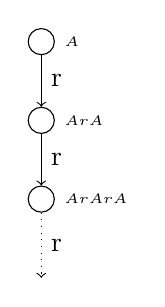
\begin{tikzpicture}
      \path{
        node[circle, draw, label=right:{\tiny$A$}] (A1) at (0,0) {}
        node[circle, draw, label=right:{\tiny$A r A$}]
        (A2) at (0,-1) {}
        node[circle, draw, label=right:{\tiny$A r A r A$}]
        (A3) at (0,-2) {}
        node[coordinate] (and so on) at (0,-3) {}
        %% 
        (A1) edge[->] node[midway, auto] {r} (A2)
        (A2) edge[->] node[midway, auto] {r} (A3)
        (A3) edge[dotted, ->] node[midway, auto] {r} (and so on)
      };
    \end{tikzpicture}
  \end{center}
  where the path to which every node corresponds is depicted right of the node.  Then, for
  $d = 3$, the unravelling of $G_C$ up to depth $3$ would just be the graph
  \begin{center}
    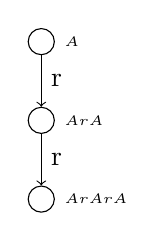
\begin{tikzpicture}
      \path{
        node[circle, draw, label=right:{\tiny$A$}] (A1) at (0,0) {}
        node[circle, draw, label=right:{\tiny$A r A$}]
        (A2) at (0,-1) {}
        node[circle, draw, label=right:{\tiny$A r A r A$}]
        (A3) at (0,-2) {}
        %% 
        (A1) edge[->] node[midway, auto] {r} (A2)
        (A2) edge[->] node[midway, auto] {r} (A3)
      };
    \end{tikzpicture}
  \end{center}
  and the corresponding \ELbot concept description is
  \begin{equation*}
    C_3 = \exists r. \exists r. \exists r. \top.
  \end{equation*}
\end{Example}

\todo[inline]{Write: unravelling}%

%%% Local Variables: 
%%% mode: latex
%%% TeX-master: "../main"
%%% End: 

%  LocalWords:  Prediger
